\subsection{Galería: barbas famosas en retratos de época}
\label{sec:galeria}

Las barberías clásicas tienen la pared llena de retratos de cortes y barbas. La Galería, dentro de \emph{Estilos}, hace lo mismo con siete retratos de dominio público de Wikimedia Commons: Lincoln (barba de candado sin bigote, 1863), Marx (barba completa larga, 1875), Twain (bigote de morsa, 1907), Douglass (melena y barba corta, c.~1879), el autorretrato de Van Gogh (barba pelirroja, 1887), Einstein (pelo despeinado y bigote, 1947) y Nietzsche (bigote manubrio, 1882). Tu cara entra al cuadro y te quedas con la barba del retrato; la app dice qué pedirle al barbero y descarga el retrato enmarcado con una placa: «Kalos como Karl Marx». Los créditos de cada retrato están en \archivo{frontend/assets/galeria/CREDITOS.md}.

\begin{figure}[htbp]
  \centering
  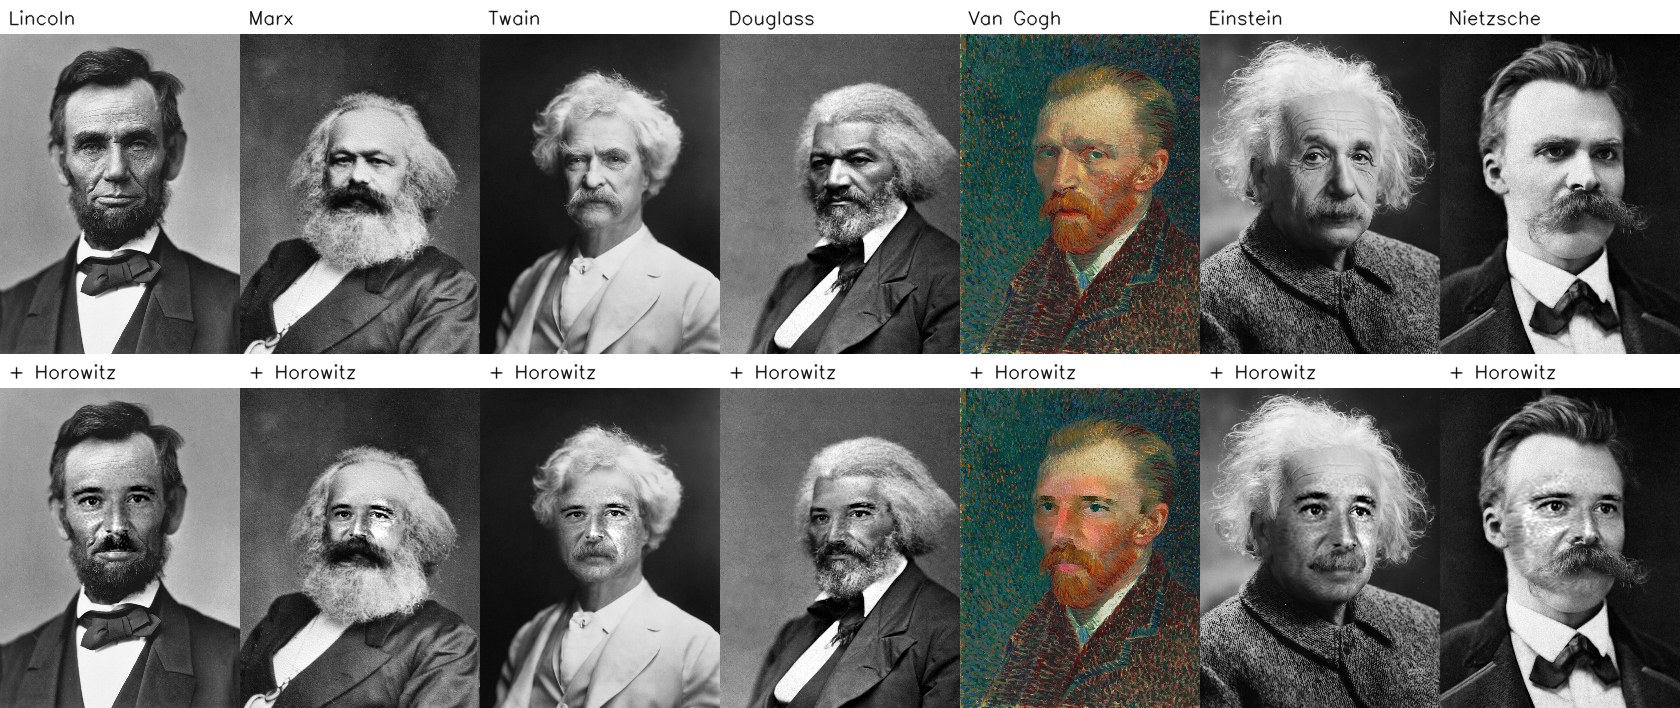
\includegraphics[width=\linewidth]{galeria.jpg}
  \caption{Arriba, los siete retratos de la Galería. Abajo, la cara de un retrato de la NASA dentro de cada uno: la barba y el bigote del retrato quedan encima, las fotos antiguas vuelven la cara blanco y negro, y el autorretrato de Van Gogh la repinta.}
  \label{fig:galeria}
\end{figure}

\textbf{Preparación de los retratos.} \archivo{backend/training/gallery.py} recorta cada original a un busto 3:4 de $900\times1200$~px (la cara ocupa un tercio del ancho y los ojos quedan al 40~\% del alto), calcula su malla de 468 puntos y dibuja la zona de vello que debe quedar encima de la cara del visitante. Esa zona se arma con las regiones de barba que ya usa la app (barba completa, bigote, boca) sobre los 68 puntos del retrato, y se agranda con un factor de ancho y alto elegido a ojo para cada barba: el bigote de Nietzsche, por ejemplo, ocupa casi el ancho de la cara. Se guarda una vez, porque los retratos no cambian.

\textbf{Composición.} Es el mismo cambio de cara de Fiesta (sección~\ref{sec:fiesta}), con el retrato como destino y la foto del visitante como donante, y tres cambios:
\begin{itemize}
  \item la máscara se multiplica por $1-v$, donde $v$ es la zona de vello del retrato: la barba y el bigote originales quedan encima;
  \item si el retrato es blanco y negro o sepia (la desviación de los canales $a$ y $b$ de CIELAB suma menos de 6), la transferencia de Reinhard puede bajar la variación de color hasta cero, así que la cara queda en el tono del retrato; además se suaviza un poco y recibe el grano de la propia foto, es decir, su detalle más fino $T = R - G_\sigma * R$ con $\sigma$ de un cuatrocientosavo del ancho de cara;
  \item la variación de luminosidad puede crecer hasta 2,5 veces, para que una foto de webcam oscura no quede gris dentro de un retrato con buen contraste.
\end{itemize}

\textbf{Filtro de Kuwahara.} En la pintura, la cara se repinta con el filtro de Kuwahara \cite{kuwahara1976}, un algoritmo de \emph{render} no fotorrealista que da aspecto de óleo y respeta los bordes. Alrededor de cada píxel hay cuatro ventanas cuadradas de lado $a+1$, una por esquina; el píxel toma el color medio de la ventana cuyo brillo varía menos:
\begin{equation}
  I'(p) = \mu_{k^\ast}(p), \qquad k^\ast = \arg\min_{k\in\{1,2,3,4\}} \sigma^2_k(p).
\end{equation}
Como en una zona plana todas las ventanas dan lo mismo y junto a un borde gana la que no lo cruza, el resultado son pinceladas de un color sin borrar los contornos. Las medias y varianzas de todas las ventanas salen de tablas de áreas sumadas (imágenes integrales) \cite{crow1984}: cada suma es $S = T(x_1,y_1) - T(x_0,y_1) - T(x_1,y_0) + T(x_0,y_0)$, así que el costo no depende de $a$. El radio es un cuarentavo del ancho de cara, y encima se suma el detalle fino del propio cuadro para que la cara tenga las pinceladas del mismo pincel.

\textbf{Interfaz y tiempos.} El botón «Entrar a los 7 cuadros» manda una foto y recibe los siete retratos en unos 1,5~s (entre 0,1 y 0,4~s cada uno; el de Van Gogh es el más lento por el filtro). La descarga arma en el navegador un \emph{canvas} con marco, paspartú y la placa de bronce. \archivo{backend/tests/test_gallery.py} tiene 6 pruebas: el catálogo y sus archivos, la detección de retratos monocromos, que Kuwahara deja igual una zona plana y no cruza un borde, que la barba de Marx queda intacta en el resultado y la API.
